\documentclass[11pt]{article}
%\usepackage[brazil]{babel}
%\usepackage[latin1]{inputenc}
\usepackage{lscape,graphicx,url}
\usepackage[utf8]{inputenc}
\usepackage{algorithm}
\usepackage{algorithmic}
\usepackage[fleqn]{amsmath}
\usepackage{amssymb}
\usepackage{amsfonts}
\usepackage{amssymb}
\usepackage{anysize}
\usepackage{placeins}
\usepackage{color, colortbl}
\usepackage{hyperref}
\usepackage{multirow}
\usepackage{rotating}

\newcommand{\red}[1]{{\color{red}{#1}}}

\marginsize{2cm}{2cm}{2cm}{2cm}

\title{Cloze questions generator\\ \bf{User manual}}

\author{Cristiano Arbex Valle}
\date{}

\begin{document}

\maketitle

This document explains how to use the Python3 script \texttt{clozeQuestionGenerator.py} to create a Cloze question in Moodle with possibly multiple variants and automatic penalties for correct answers of the wrong variant. The user is required to write a text file containing some parameters, the question text in Latex and the variant values (both answers and varying parameters). The script generates a Moodle XML file that can be directly imported into Moodle.

\section{The input file}

The example below shows a basic text file used as input to the script.

\begin{verbatim}
# This is a comment
CategoryName     Prova XX/Questoes AA
QuestionName     Questão de teste
QuestionWeights  1 1 2
VariantPenalty   200
Tolerance        0.001 0.001 0.001

QuestionText

Considere a função $f(x) = @x^2 - 6x + 3$. Responda as questões a seguir.

Qual é o valor do discriminante na fórmula de Bhaskara, $b^2 - 4ac$? *

Qual é a menor raiz da equação? *

Qual é a maior raiz da equação? *

Resolva com três casas decimais. Se errar perde R\$10. Dica: a maior raiz está entre @ e @.

EndQuestionText

Variants
1,0 24 0,551 5,449 4 6
1,5 18 0,586 3,414 3 5
2,0 12 0,634 2,366 2 4
2,5  6 0,710 1,690 1 3
3,0  0 1,000 1,000 0 2
EndVariants
\end{verbatim}

\subsection{General parameters}

Lines starting with \# are treated as comments and are ignored by the script. The parameters in the example above follow a certain order, but they can be defined in any order, including after the quesion text and variant values.

A line that starts with {\bf CategoryName} defines the category in which the question will be placed in. This field is mandatory. By using a slash (/), nested categories can be automatically created. For instance, in the example above the questions will be placed under category \texttt{Questoes AA} inside another category \texttt{Prova XX}. The parameter {\bf QuestionName} is also mandatory.

A question can have multiple parts. In that case, the user can optionally assign different weights to each part. In the example above, the user must answer three parts. In the parameter {\bf QuestionWeights} in the example, the first two parts get weight 1 and the last (third) part gets weight 2 (so twice the value of the other questions). Due to a Moodle limitation the weights must be integers. If the {\bf QuestionWeights} are not provided, all parts get the same weight by default.

A question can have multiple variants, that is, different answers to questions with different values. If desired, the student can be penalised by giving a correct answer to the wrong variant. This helps in, for instance, automatically punishing students who copy questions from classmates. To assign such punishment, the user must define the {\bf VariantPenalty} parameter. It must also be an integer number due to a Moodle limitation and it is given as a percentage. In the example above, the value 200 means that if the student gives the correct answer of a wrong variant it receives a -200\% penalty when Moodle automatically evaluates the question.

The final parameter in the example before the actual question text is {\bf Tolerance}. It defines the error tolerance regarding the right answer for each of the three parts. If only a single value is provided after {\bf Tolerance}, then the same tolerance is applied to all parts (if applicable). If no Tolerance is provided, the default tolerance is zero for integers and 0.1 for answers with one decimal place, 0.01 for questions with two decimal places, etc.

\subsection{Question text}

The next step in the example above is defining the question text. The question text must start after a line containing only {\bf QuestionText} and nothing else, and it ends when a line containing {\bf EndQuestionText} is found (and nothing else). This is mandatory. 

The question text accepts a limited selection of Latex code - anything outside the scope presented here is not guaranteed to be bug-free. Mathematical notation must be defined between single dollar signs (\$). In the output XML file, the dollar signs are automatically replaced by \textbackslash( and \textbackslash). If the user wishes to replace it to \$\$ instead, just open the python script and change variables \texttt{latexBegin} and \texttt{latexEnd}. If the user wants to include the symbol \$ in the text unrelated to Latex, then it must be escaped as \textbackslash\$. This can be seen in the last line of the example above.

Currentl

There are two types of wildcards. The symbol @ is used to define parameters in the question that may vary according to different variants. In the example above there are three instances of @. The wildcard * defines a part of the question the must be answered by the student. In the example above there are also three of them. Every question must have at least one wildcard *. Parameter wildcards @ are optional. Since the symbols @ and * are reserved, they cannot be used in the question text. If the user wishes to replace the symbols used as wildcards, change the variables \texttt{parameterIdentifier} and \texttt{questionIdentifier} in the script. Notice that wildcards must be composed of a single symbol.

\subsection{Variants}

In the example above, the last commands defined the variant values. A line containing the text {\bf Variants} (and nothing else) marks the beginning of it and a line containing {\bf EndVariants} (and nothing else) marks the end. At least one variant value is mandatory. Each line contains the values (must be numerical) for both wildcards in the order that they appear. In the example above there are 6 different variants. For instance, in the first line the value 1,0 is used to replace $f(x) = @x^2 - 6x + 3$ (the first wilcard). The next three values (24, 0,551 and 5,449) represent the solutions to the questions (as defined by wildcards *). Finally the last two numbers, 4 and 6, are used to replace the two parameter wildcards in \textit{a maior raiz está entre @ e @}.


\section{A second example}

\begin{verbatim}
CategoryName     Prova XX/Questoes BB
QuestionName     Questão de teste 2
VariantPenalty   1
Tolerance        0.0005

QuestionText
Conhecemos estes pontos da curva da função $f$:

$\begin{array}{cc}x & f(x)\\ 
\hline 
1,41658 & @ \\ 
1,6762  & @ \\ 
2,98006 & @ \\ 
4       & @ \\ 
5,01994 & @ \\ 
6,3238  & @ \\ 
6,58342 & @
\end{array}$

A quadratura de Gauss-Legendre com três pontos fornece qual aproximação de $\int_1^7 f$? 
\textit{Usar 5 casas} {\it decimais.}

*

\textbf{Dica para}  {\bf verificação:} o resultado está entre 
52 e 54. \textbf{\textit{Testando itálico e negrito juntos.}}
EndQuestionText

Variants
1,97443 2,40622 5,27052 8,10226 11,34185 15,99721 16,98726 52,27869
1,9886  2,42299 5,30033 8,14226 11,39205 16,06045 17,0531  52,51869
2,00277 2,43975 5,33013 8,18226 11,44225 16,12369 17,11893 52,75869
2,01693 2,45651 5,35993 8,22226 11,49245 16,18693 17,18477 52,99869
2,0311  2,47327 5,38973 8,26226 11,54265 16,25017 17,2506  53,23869
EndVariants
\end{verbatim}

The example above includes latex arrays for matrix representation, including linebreaks (\textbackslash\textbackslash) and ampersands (\&). It also employs italics and bold using commands \texttt{\textbackslash textbf\{\}} and \texttt{\{\textbackslash bf\}}, \texttt{\textbackslash textit\{\}} and \texttt{\{\textbackslash it\}}. So far only these commands are accepted. There is no support for different colours or different text highlights at the moment.

\section{Running the script}

To run the script, simply do:

\begin{verbatim}
python3 clozeQuestionGenerator.py example1.txt example1.xml
\end{verbatim}

\noindent or whichever is the python command you use. The second argument, \texttt{example1.txt} is the name of the text file containing the first example, and the second argument must be a file ending with \texttt{.xml}. In the example above the file \texttt{example1.xml} will be created and it can be imported straight into Moodle.


\section{Importing a question}

Once a XML file is generated, you can import it into Moodle. To import a file, just follow Figure \ref{fig1} and make sure that the selected format is \texttt{Moodle XML}. Choose the XML file and  you are ready to go.

\begin{figure}[!htb]
\centering
  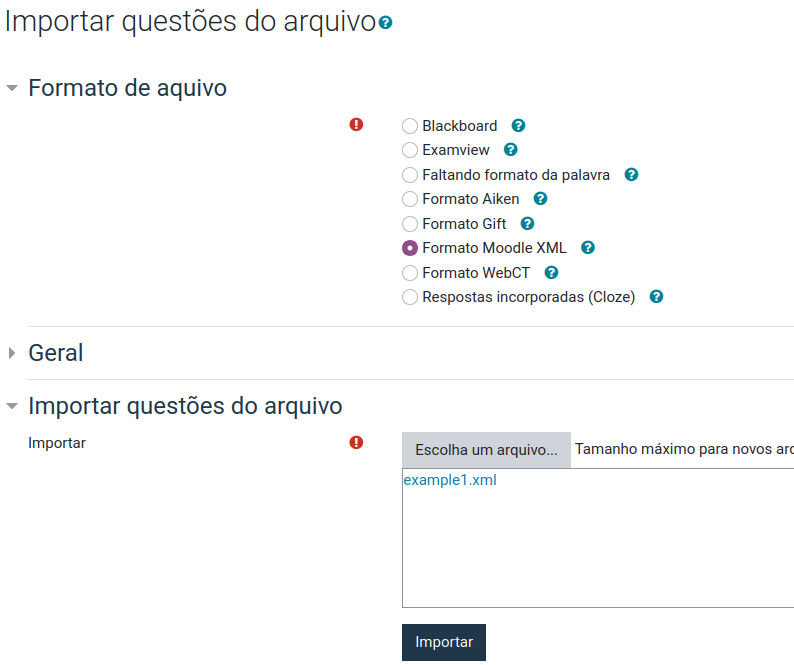
\includegraphics[width=0.8\textwidth]{figures/importing.png}
  \caption{Importing a XML file into Moodle}
  \label{fig1}
\end{figure}

After importing it you will be redirected to the screen containing the question, as shown in Figure \ref{fig2}. Notice that if multiple variants are used, names V.1, V.2, etc. are added automatically to the end of the {\bf QuestionName} defined in the input file. Also notice how the properly nested categories have been created automatically. A visualization of one of the questions is shown in Figure \ref{fig3}

\begin{figure}[!htb]
\centering
  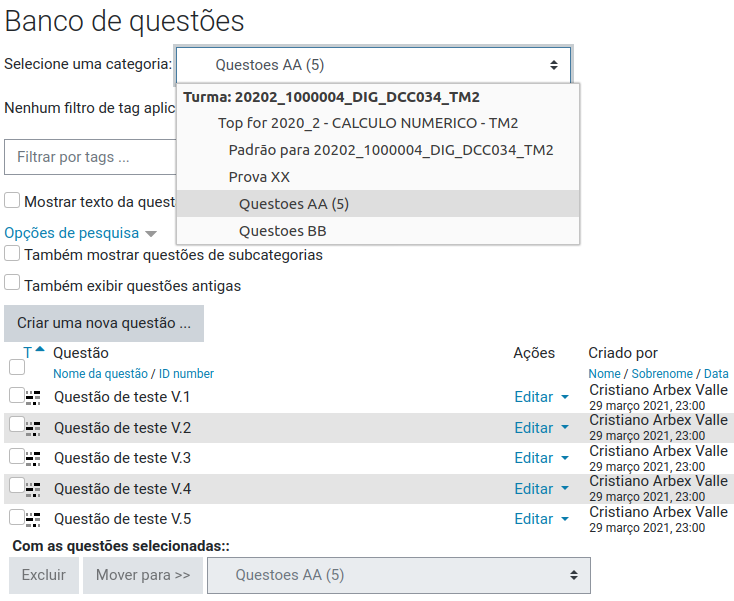
\includegraphics[width=0.9\textwidth]{figures/questoes.png}
  \caption{Questions imported into Moodle}
  \label{fig2}
\end{figure}


\begin{figure}[!htb]
\centering
  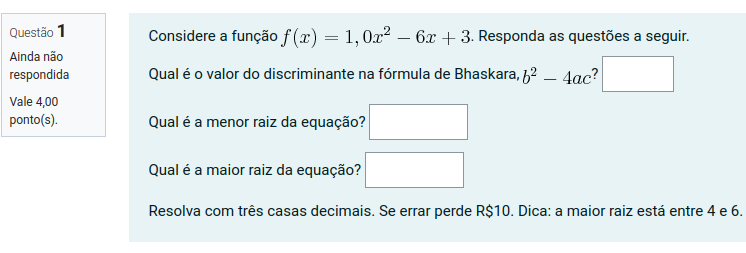
\includegraphics[width=1\textwidth]{figures/exemplo.png}
  \caption{Visualizing an imported question}
  \label{fig3}
\end{figure}




\end{document}
